\subsection{Clasificación}

		Como explica de manera sencilla Murphy K. P. en \cite{Murphy12}, el objetivo del aprendizaje supervisado es aprender un mapeo desde las entradas $x$ a las salidas $y$. En clasificación, $y_i \in \{1,\dots,C\}$ con $C$ siendo el número de clases. Si $C=2$, estamos frente al problema de \textit{clasificación binaria}; mientras que si $C>2$, la clasificación pasa a ser \textit{multiclase}. Existe otro tipo de clasificación denominada \textit{clasificación multi-etiqueta}, que difiere de la multiclase en cuanto a que las clases no son mutuamente excluyentes, es decir, una muestra puede pertenecer a dos o más categorías o clases. En este último caso, el mapeo se realiza desde la entrada $x$ a un vector $z$, más que a una salida escalar. La elección de cual usar esta directamente asociada al tipo de problema que se quiera resolver.
		
		Tal como expresa P. Domingos en \cite{PDomingo} el objetivo del aprendizaje automático es \textit{generalizar} más allá de los ejemplos en el conjunto de entrenamiento. Ya que, no importa cuantos datos tengamos, es muy poco probable que vayamos a ver los mismos ejemplos al momento de evaluar.
		
		Para Murphy, una manera de formalizar el problema es a partir de una función de aproximación. Se asume $y = f_{\theta}(x)$ para cierta función desconocida $f_{\theta}$, y el objetivo del aprendizaje es estimar los parámetros $\theta$ de la función $f$ dado un conjunto de entrenamiento etiquetado. Posteriormente, se realizan predicciones usando $\hat{y} = f_{\hat{\theta}}(x)$ (usamos el símbolo \string^ para denotar estimación). El objetivo principal es realizar predicciones en entradas nuevas, es decir, que no se hayan visto durante el entrenamiento.
		
		%En esta sección, se procede a explicar en detalle el clasificador \textit{Random Ferns}. Se van a detallar otros clasificadores como Na\"{i}ve Bayes, árboles de decisión y Random Forest que son necesarios para poder comprender la elección de Random Ferns. 
		
		
	\subsubsection{Clasificadores Probabilísticos}

		Los clasificadores probabilísticos determinan, dada una entrada nueva, la probabilidad de que esta pertenezca a un conjunto de clases, a diferencia de otros clasificadores, que simplemente predicen a que clase pertenece la misma. Esto lo realiza asignando una distribución de probabilidad al conjunto de clases.
	
	Formalmente un clasificador probabilístico es una distribución condicional $p(Y|X)$ sobre un conjunto finito de clases $Y$ dada $X$ entradas. Una forma de determinar cual es la mejor clase $\hat{y} \in Y$ para $X$ sería elegir la clase con la probabilidad más alta
	$$\hat{y} = argmax_{y}p(Y=y|X) $$
	
	Uno de los clasificadores más populares es \textit{na\"{i}ve Bayes} (que se procede a explicar en las próximas secciones). Este clasificador junto con el resto, derivan de modelos de probabilidad generativos que proporcionan un principio para el estudio de la clasificación estadística en dominios complejos tales como el lenguaje natural y el procesamiento visual \cite{GargRo01}.


	\subsubsection{Teoría de decisión}
	
	La teoría de decisión nos ayuda a tomar decisiones óptimas en situaciones que involucran incertidumbre. La incertidumbre hace referencia a un estado de conocimiento limitado donde es imposible describir con exactitud el estado existente, la salida futura, o más de una posible salida.
	
	Supongamos que tenemos un vector $x$ como entrada junto con el correspondiente vector $t$ de variables objetivo, la meta es predecir $t$ dado un nuevo valor de $x$. En problemas de regresión, $t$ comprenderá variables continuas, mientras que en problemas de clasificación $t$ representará etiquetas de clase. La determinación de la probabilidad conjunta de $x$, $t$ denotada como $p(x,t)$ dado un conjunto de datos de entrenamiento es un ejemplo de \textit{inferencia} y es típicamente un problema muy difícil. La inferencia, en este caso, hace relación a la estadística inferencial la cual es una parte de la estadística que comprende los métodos y procedimientos que por medio de la inducción determina propiedades de una población estadística, a partir de una pequeña parte de la misma.
	
	Consideremos el siguiente ejemplo, sea $C=\{C_1,\dots,C_k\}$ un conjunto de etiquetas de clase, sea $t \in C$ y sea $x$ un vector de entrada nuevo. Se desea determinar a que clase pertenece $x$. El problema de inferencia involucra determinar la distribución conjunta $p(x,C_k)$, o equivalentemente $p(x,t)$.

	Como se dijo anteriormente, el objetivo es decidir a cual de las $k$ clases pertence el vector de entrada $x$ . Estamos interesados entonces, en las probabilidades de las $k$ clases dado $x$, es decir $p(C_k|x)$, $k=1,\dots,K$. Usando el Teorema de Bayes, estas probabilidades pueden expresarse de la forma:
		\begin{align*}
			p(C_k|x) = \frac{p(x|C_k)p(C_k)}{p(x)}
		\end{align*}

	Ahora podemos interpretar $p(C_k)$ como la probabilidad a priori para la clase $C_k$, y $p(C_k|x)$ como la correspondiente probabilidad a posteriori. Por ejemplo, $p(C_1)$ representa la probabilidad de pertenecer a la clase $C_1$, antes de observar la muestra $x$
	
	Se pueden distinguir dos etapas en el problema de clasificación, la \textit{etapa de inferencia} en el cual se usan los datos para entrenar el modelo para $p(C_k|x)$, y la subsecuente \textit{etapa de decisión} en la cual se usan las probabilidades a posteriori para poder realizar asignaciones óptimas de las clases. Una alternativa, es la de resolver ambos problemas en conjunto y simplemente entrenar una función que mapee las entradas $x$ directamente con las decisiones. Dicha función es llamada \textit{función discriminante}.
	
	De hecho, se pueden identificar tres enfoques diferentes al momento de resolver problemas de decisión. En orden decreciente de complejidad, estos son:
		\begin{enumerate}
			\item Primero, resolver el problema para determinar las densidades condicionales $p(x \vert C_k)$ para cada clase $C_k$ individualmente. También de forma separada, inferir las probabilidades de clases a priori $p(C_k)$. Después, usar el teorema de Bayes en la forma:
			$$p(C_k \vert x) = \frac{p(x \vert C_k)p(C_k)}{p(x)} $$
			para encontrar las probabilidades a posteriori $p(C_k \vert x)$. Como es usual, el denominador en el teorema de Bayes puede ser encontrado en término de las cantidades que aparecen en el numerador, como:
			 $$p(x) = \sum_k p(x \vert C_k)p(C_k) $$
			Equivalentemente, se puede modelar la distribución conjunta $p(x,C_k)$ directamente y después normalizar para obtener las probabilidades a priori. Habiendo encontrado las probabilidades a posteriori, se puede usar la teoría de decisión para determinar la pertenencia a una clase para cada entrada nueva $x$. Los enfoques que explícitamente o implícitamente modelan la distribución de las entradas así también como las salidas son conocidos como \textit{modelos generativos}, debido a que tomando muestras de ellos es posible generar puntos de datos sintéticos en el espacio de entrada.
			\item Primero, resolver el problema de inferencia para determinar las  probabilidades de clase a posteriori $p(C_k \vert x)$, y luego subsecuentemente usar la teoría de decisión para asignar a cada $x$ nueva una de estas clases. Los enfoques que modelan las probabilidades a posteriori directas son llamados \textit{modelos discriminativos}.
			\item Encontrar una función $f(x)$, llamada función discriminante, que mapea directamente cada entrada $x$ con una etiqueta de clase. Por ejemplo, en el caso del problema de dos clases, $f(\cdot)$ puede ser valuada de manera binaria, de manera que $f = 0$ represente a la clase $C_1$ y $f = 1$ represente a la clase $C_2$. En este caso, las probabilidades no toman partido. 
		\end{enumerate}
		
	Consideremos los méritos relativos a estas tres alternativas. El enfoque (1) es el más demandante debido a que involucra encontrar la distribución conjunta tanto de $x$ como de $C_k$. Para muchas aplicaciones, $x$ tendrá alta dimensionalidad, y por consiguiente puede ser necesario un conjunto de entrenamiento grande con el fin de ser capaz de determinar las densidades de clase condicional con una exactitud razonable. Hay que tener en cuenta que la probabilidades a prior $p(C_k)$ de la clase a menudo pueden estimarse simplemente a partir de las proporciones de los punto de datos del conjunto de entrenamiento en cada una de las clases.
		
	Sin embargo, si sólo deseamos realizar decisiones de clasificación, esto conlleva a un gasto de recursos computacionales y una demanda de datos excesiva para encontrar la distribución conjunta $p(x, C_k)$ cuando de hecho, solamente se necesitan las probabilidades a posteriori $p(C_k \vert x)$, las cuales pueden ser obtenidas a través del enfoque (2). 
		
	Un enfoque mucho más simple es (3) en el cual se usa una conjunto de entrenamiento para encontrar una función discriminante $f(x)$ que mapea cada $x$ directamente a una etiqueta de clase, así combinando la inferencia y las etapas de decisión en un simple problema de aprendizaje.
		
	Con la opción (c), sin embargo, se pierde el acceso a las probabilidades a porteriori $p(C_k \vert x)$. 
	
	\subsubsection{Vectores de características} \label{subsec:feature}

	Un característica o feature, es un aspecto o cualidad distintiva de un objeto (clase de interés). Las características son importantes dado que al representar los aspectos o cualidades mas significativas de un objeto, facilitan el reconocimiento posterior de objetos similares. Esto es fundamental por ejemplo, en los esquemas de clasificación en el aprendizaje supervisado ya que permite, dada una muestra desconocida, identificar a que clase pertenece si anteriormente sabemos las características particulares de cada clase (a partir de instancias o muestras analizadas con anterioridad). Esto conlleva a que si se realiza una buena selección de características, impacte positivamente en la precisión de los clasificadores y por ende en el reconocimiento. Por ejemplo, en los algoritmos de detección de spam, las características pueden incluir el lenguaje en el que esta escrito el email, la ausencia o presencia de ciertos encabezados, la corrección gramatical del texto, entre otros~\cite{SpamPaper}.

	Un vector de características o ``feature vector'', es un  vector $n$-dimensional de características numéricas que se diseña de forma tal de conjeturar propiedades características de los objetos. Muchos algoritmos en machine learning requieren la representación numérica de los objetos, dado que dichas representaciones facilitan el análisis estadístico y el procesamiento de los datos.
		
	
		
	

	
	\subsubsection{Clasificador Na\"{i}ve Bayes}

	Es un clasificador probabilístico basado en la aplicación del teorema de Bayes con una fuerte suposición de independencia (na\"{i}ve). En términos simples, un clasificador na\"{i}ve Bayes asume que la presencia o ausencia de una característica particular no está relacionada con la presencia o ausencia de cualquier otra característica. Este tipo de clasificador considera que cada una de estas características contribuye independientemente a la probabilidad de que un elemento sea de una clase particular, independientemente de la presencia o ausencia de otras características. Por ejemplo, una fruta puede ser considerada una manzana si es roja, redonda y de 7cm de diámetro aproximadamente.

	El modelo para un clasificador es:
		$$p(C \vert F_1,\dots,F_n)$$
	sobre una variable dependiente C, con un pequeño número de resultados (o clases). Esta variable está condicionada por varias variables independientes (\textit{features}) desde $F_1$ a $F_n$. El problema es que si el número $n$ de variables independientes es grande (o cuando éstas pueden tomar muchos valores), entonces basar este modelo en tablas de probabilidad se vuelve computacionalmente imposible ya que, por ejemplo, si hubiesen $35$ variables independientes con $2$ valores posibles cada una entonces habrían $34.359.738.368$ valores posibles distribuidos en múltiples tablas. Si se usaran decimales de punto flotante simple (4 bytes), se necesitarían 32 gigabytes de memoria para almacenar todo, lo que lo hace muy poco manipulable. Por lo tanto el modelo se reformula para hacerlo más manejable:
Usando el teorema de Bayes se escribe:
		\begin{align*}
		p(C \vert F_1,\dots,F_n) = \frac{p(C) \ p(F_1,\dots,F_n\vert C)}{p(F_1,\dots,F_n)}.
		\end{align*}
		que puede ser reescrita como sigue, aplicando repetidamente la definición de probabilidad condicional:
		\begin{align}
		p(C, F_1, \dots, F_n)
		&= p(C) \ p(F_1,\dots,F_n\vert C) \\
		&= p(C) \ p(F_1\vert C) \ p(F_2,\dots,F_n\vert C, F_1) \\
		&= p(C) \ p(F_1\vert C) \ p(F_2\vert C, F_1) \ p(F_3,\dots,F_n\vert C, F_1, F_2)
		\end{align}
		y así sucesivamente. Ahora es cuando la asunción "na\"{i}ve" de independencia condicional entra en juego: se asume que cada $F_i$ es independiente de cualquier otra $F_j$ para $j \neq i$. Esto significa que
		\begin{align*}
		p(F_i \vert C, F_j) = p(F_i \vert C)
		\end{align*}
		por lo que la probabilidad compuesta puede expresarse como
		\begin{align*}
		p(C, F_1, \dots, F_n) 
		&= p(C) \ p(F_1\vert C) \ p(F_2\vert C) \ p(F_3\vert C) \dots \\
		&= p(C) \prod_{i=1}^n p(F_i \vert C).
		\end{align*}
		Esto significa que haciendo estas presunciones, la distribución condicional sobre C puede expresarse de la siguiente manera:
		$$p(C \vert F_1,\dots,F_n) = \frac{1}{Z}p(C)\prod_{i=1}^n p(F_i \vert C)$$
		donde $Z$ es un factor que depende sólo de $F_1,\dots , F_n$, es decir, constante si los valores de $F_i$ son conocidos.
		
	
	\subsubsection{Árboles de decisión}
\label{subsection:arboles_decision}

%	Desde el punto de vista de las ciencias de la computación y las matemáticas, un árbol es un grafo conexo simple y sin ciclos, y sus propiedades son básicas de la teoría de grafos. Formalmente, un grafo es una estructura de la forma $G=(V,E)$, donde $V$ es un conjunto de vértices o nodos y $E=\{ (v_i, v_j), v_j,v_i \in V \}$ es un conjunto de pares donde cada par representa una arista o rama que conecta a dos nodos.

%	Además, definimos un \textit{camino} o \textit{path} entre los nodos $v_i, v_j \in V, i \neq j$ en $G$ (lo denotamos $P_{v_i, v_j}^G$), como el conjunto $\{ v_i, v_{i+1}, \dots, v_{j-1}, v_j \}$ de nodos talque  $(v_k, v_{k+1}) \in E, k = i, \dots, (j-1)$. Luego, decimos que $G$ es conexo si $\forall v_i, v_j \in V, i \neq j, \exists P_{v_i, v_j}^G$ y no tiene ciclos si $\forall v_i, v_j \in V, i \neq j, \exists ! P_{v_i, v_j}^G $.

	%En un árbol existen dos tipos de nodos. La diferencia radica en la cantidad de nodos adyacente al mismo o grado del nodo, que se denota como $d(v_i), v_i \in V$. Los nodos con grado $\leq 1$ se denominan hojas y el resto son nodos internos. Los árboles que se consideran en este trabajo tienen un tercer tipo de nodo que llamamos raíz y es único. Los árboles con raíz son muy comunes en el área de aprendizaje automático y formalmente se pueden definir en términos de \textit{generaciones} o \textit{niveles}. Es decir, se toma al nodo raíz como el nivel 0, los vecinos del mismo constituyen el primer nivel y los que están a distancia $k$, forman el $k$-esimo nivel.

	Un árbol de decisión es una estructura jerárquica compuesta por nodos internos que representan evaluaciones sobre ciertos atributos, características del problema que se busca resolver, y nodos hoja que representan las decisiones finales en base a las evaluaciones de los nodos. La rama que conecta a un par de nodos refleja uno de los posible valores para el atributo del nodo padre.
	
	Los árboles, en el área de la computación, son estructuras de datos capaces de almacenar y representar información de forma jerárquica (a través de sus nodos). En general y en especial en el área de aprendizaje supervisado son de mucha utilidad ya que computacionalmente son eficientes a la hora de buscar información dentro de ellos (a diferencia de otras estructuras de datos). Además, su representación es fácil de interpretar y su implementación es sencilla.

	Consideremos la Figura \ref{fig: Arbol de decision} que contempla el siguiente ejemplo: ¿Es conveniente ir a jugar al tenis basado en las condiciones climáticas?. La figura es una representación de un árbol de decisión que tiene un estructura similar a un diagrama de flujo. Como se puede observar, en cada nodo del árbol se evalúa un atributo diferente. En este caso, cada atributo hace referencia a una condición climática. En base a las respuestas de los nodos, se avanza en el árbol hasta llegar a una hoja donde se toma una decisión. En el ejemplo de la figura, si el clima está despejado y la humedad es normal entonces es conveniente ir a jugar al tenis. Los árboles de decisión pueden ser usados para la clasificación, variables discretas, o regresión, variables continuas. Cuando son usados para la clasificación, cada nodo representa una característica, cada rama que sale de un nodo representa un valor posible para la característica que representa al mismo y por último las hojas representan la etiqueta de clase (decisión tomada luego de computar todos los nodos). La clasificación comienza en la raíz, donde se pregunta sobre algún valor de una característica en particular del objeto a analizar. Las diferentes ramas que salen de la  raíz corresponden a las diferentes valores posibles. Basado en la respuesta, se continúa por la rama hasta el nodo siguiente. La siguiente etapa, es realizar una decisión en el nodo en cuestión que puede ser considerado como la raíz del sub-árbol y se continua de esta manera hasta que se alcanza una hoja, la cual no contiene más preguntas. Cada hoja contiene una etiqueta categórica y al objeto, se le asigna la etiqueta de la hoja que ha alcanzado.
	
		\begin{figure}[htbp]
			\centering
			\fbox{ 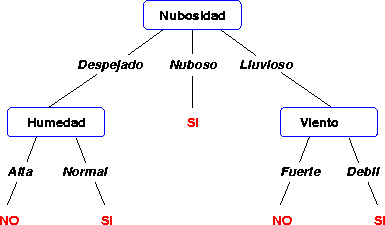
\includegraphics[scale=0.5]{img/tenis_decision_tree.png} }
			\caption[Árbol de decisión]{Árbol de decisión. Imagen extraida de Mitchell, T.M. (1997) \textit{Machine Learning}, McGraw-Hill.}
			\label{fig: Arbol de decision}
		\end{figure}
		
	Los algoritmos para entrenar un árbol de decisión usualmente trabajan de \textit{arriba hacia abajo}(\textit{top-down}, por su denominación en inglés) \cite{LROM05}. Dado un conjunto de características iniciales, en cada nodo del árbol, los algoritmos utilizan una función que evalúa cúal es el atributo más apropiado para representar al nodo y en base a eso dividen el conjunto inicial en dos o más partes. La elección de que función utilizar para realizar estas decisiones no es sencilla. En algunos casos, lo que se busca es generar un árbol de decisión óptimo que reduzca el error de generalización, en otros, se busca reducir el número de nodos o la profundida del árbol \cite{LROM10}. Este proceso continúa de manera recursiva hasta que el subconjunto de características en un nodo tiene el mismo valor para la variable objetivo, sea una clase o un valor numérico, o cuando las divisiones no agregan ningún valor a las predicciones. Este proceso es una estrategia muy común al momento de entrenar un árbol de decisión a partir de datos y es un ejemplo de \textit{algoritmo ambicioso}(\textit{greedy algorithm}, por su traducción al inglés). Si se considera nuevamente el ejemplo de la Figura \ref{fig: Arbol de decision}, se puede ver que los atributos, si bien son pocos, están bien ubicados en los nodos del árbol. En cambio, si se intercambian los nodos con los atributos \textit{humedad} y \textit{viento}, entonces el preguntar por la humedad sabiendo que el día está lluvioso no aporta información al momento de tomar una decisión.
	
	Cada algoritmo tiene su propio método al momento de dividir los nodos y decidir cuál es la mejor división que conlleve a disminuir los errores de clasificación. Por ejemplo, los algoritmos \textit{ID3 y C4.5}, \cite{QuinlanID3, QuinlanC45}, el primero precursor del segundo, utilizan el concepto de \textit{entropía} o \textit{entropía de información} para elegir al atributo que va a dividir el conjunto de características y que obviamente va a representar al nodo en el árbol. La entropía se la define como la medida de incertidumbre de una variable aleatoria.  Básicamente, dado un conjunto de características $S$, se itera sobre cada atributo no usado del mismo y se calcula la entropía sobre el mismo de la siguiente manera:
	\begin{align}
		\eta(S) = -\sum_i P(s_i)log_{2}P(s_i)
	\end{align}
	donde $S$ es nuestro conjunto conformado con los posibles valores $\{ s_1,\dots, s_n \}$ y $P( \cdot )$ es la función de probabilidad. Posteriormente, se elige aquel atributo que tenga menor entropía, mayor ganancia de información, y se lo utiliza para partir el conjunto $S$. Construir un árbol de decisión se basa en encontrar atributos que retornen la mayor ganancia de información con lo cual se obtienen ramas más homogéneas.
	
	Los árboles de decisión crecen hasta que se cumplen ciertos criterios: que se haya alcanzado la máxima profundidad del árbol, que todas las instancias del conjunto de entrenamiento pertenezcan a un solo valor de salida, entre otros \cite{LROM10}.

	Como expresan O. Maimon y L. Rokach en \cite{LROM10}, se puede dar el caso de que el árbol resultante sea excesivamente complejo, por ejemplo, al tener demasiados parámetros relativos al número de observaciones. Esto es lo que se conoce como \textit{sobreajuste} (\textit{overfitting}, de su traducción al inglés). Un modelo que ha sido sobreajustado, tendrá generalmente una baja tasa de predicción. Este tipo de problemas se generan cuando se eligen pobremente los criterios de parada. El caso contrario generaría árboles pequeños o débilmente ajustados. Los autores destacan que una forma de solucionar el sobreajuste es utilizando la técnica de \textit{poda} (\textit{pruning}, de su traducción al inglés). La poda reduce el tamaño de los árboles de decisión eliminando secciones del mismo que provean poca capacidad para clasificar instancias. El objetivo es tanto la reducción de la complejidad del clasificador como así también mejorar la performance a través de la reducción del sobreajuste.
	
	%La entropía, se la define como la medida de incertidumbre en una variable aleatoria y usualmente es medida en \textit{bits, nats o bans}. Para entender el concepto, consideremos el siguiente ejemplo: procedemos a tirar una moneda, si las probabilidades de que salga cara o cruz en la misma son iguales, es decir, la moneda es ``justa'' entonces decimos que la entropía es alta. Dicho de otra manera, no hay forma de predecir con anticipación cual va a ser el resultado. En cambio, si la moneda estuviese alterada y tuviese dos caras entonces la entropía es nula o cero lo cual nos quiere decir que la salida puede ser predecida perfectamente. Formalmente, se define la entropía $\eta$ de una variable aleatoria discreta $X$ con posibles valores $\{ x_1,\dots, x_n \}$ y función de probabilidad $P(X)$ de la siguiente manera:
	%\begin{align}
	%	\eta(X) = E[I(X)] = E[-ln(P(X))]
	%\end{align}
	%donde $E$ es el valor esperado e $I$ es el contenido de información de $X$ ($I(X)$ es en sí misma una variable aleatoria). Cuando se considera una muestra finita, podemos escribir:
	%\begin{align}
	%	\eta(X) = \sum_i P(x_i)I(x_i) = -\sum_i P(x_i)log_{b}P(x_i)
	%\end{align}
	%donde $b$ es la base del logaritmo usado (comúnmente se usa $2$, $10$ o el número de Euler $e$)

		
	%\subsubsection{Árbol aleatorio}

	Un árbol aleatorio o random tree, es un árbol construido al azar a
        partir de un conjunto de posibles árboles que tienen $K$
        características aleatorias en cada nodo. ``Al azar'' en este contexto
        significa que cada árbol tiene la misma chance de ser muestreado. Los
        árboles aleatorios pueden ser generados eficientemente y una
        combinación de conjuntos grandes de estos generalmente conlleva a
        modelos precisos.


        \JS{no queda claro de que se trata. Se puede desarrollar un poco mas}
		
	\subsubsection{Random Forest}

	\paragraph{Árbol aleatorio} ~\\
	
	Para comprender que es un árbol aleatorio, es necesario comprender que es un \textit{proceso estocástico}.
	
	Un proceso estocástico, es un proceso que se caracteriza por su indeterminación. Dicho de otra manera, la evolución de este, puede ir por muchos caminos posibles, incluso si conocemos el punto de partida (o condición inicial). Se diferencian de los procesos determinísticos, ya que estos últimos evolucionan de una sola manera, es decir, que no involucran la aleatoriedad en el desarrollo de los futuros estados del mismo.	
	
	Teniendo en cuenta este concepto luego, podemos decir, que un árbol aleatorio es un árbol construido a través de un proceso estocástico. Es decir, cada nodo del árbol se construye a partir de un proceso aleatorio que le asigna su valor. Dentro de los árboles aleatorios más comunes, podemos encontrarnos a  los \textit{árboles binarios} los cuales son construido insertando un nodo a la vez de acuerdo a una permutación aletoria.

	\paragraph{Random Forest} ~\\

	\textit{Random Forest} o \textit{bosque aleatorio} es un método de aprendizaje conjunto o\textit{ ensemble learning} para la clasificación o regresión. Es un clasificador que consiste en una colección de clasificadores con estructura de árbol $\{h(x,\Theta_k), k = 1,\dots\}$, donde $\{\Theta_k\}$ son vectores aleatorios independientes e identicamente distribuidos ($\Theta_k$ representa los parámetros para la construcción del $k$-esimo árbol) y $h(x,\Theta_k)$ es un clasificador donde $x$ es un vector de entrada. Luego, dada una entrada $x$, cada árbol emite un único voto para la elección de la clase más popular para $x$ \cite{Breiman01}.

	El algoritmo de entrenamiento para random forest aplica la técnica general de \textit{bootstrap aggregating}(agregación bootstrap) o \textit{bagging}(embolsado). Esta técnica fue desarrollada también por Breiman en 1996 ~\cite{LBreiman96} y es un método para generar múltiples versiones de un predictor y usar estos para obtener un predictor agregado. Para tener una idea más clara del concepto, consideremos el siguiente ejemplo basado en el trabajo de Breiman. Supongamos que tenemos $L = \{ (x_n,y_n), n = 1,\dots, N (N \in \mathbb{N}) \}$ el cual es un conjunto de aprendizaje donde $x_n$ son valores de entrada e $y_n$ son etiquetas de clase o valores numéricos. Supongamos también que tenemos una forma de generar un predictor de la forma $\varphi(x,L)$ a partir de $L$ tal que $ \varphi(x,L) = y $. Por último, supongamos que nos dan un conjunto de predictores $\{ L_k \}$ donde cada uno consiste en $N$ observaciones independiente bajo la misma distribución de $L$. El objetivo de Breiman en su trabajo, es que usando $\{ L_k \}$ se obtenga un predictor mejor que el establecido anteriormente $\varphi(x,L)$. La única restricción, es que se nos obliga a trabajar solamente con el conjunto de predictores $\{ \varphi(x, L_k)\} $.

	Para resolver este problema, Breiman estableció el siguiente criterio. Si la respuesta $y$ era un valor numérico luego, se reemplaza a $\varphi(x,L)$ por el promedio del conjunto de predicotres $ \{ \varphi(x, L_k) \} $ sobre $k$. Es decir, $\varphi_A(x) = E_L\varphi(x,L)$ donde $E_L$ denota la esperanza sobre $L$, y el subíndice $A$ en $\varphi_A$ denota la agregación. En cambio, si $\varphi(x,L)$ predecía una etiqueta de clase $j \in \{ 1,\dots, J \} $, luego un método para agregar todos los predictores era a través del voto. Es decir, para el autor $N_j = \{ k;\varphi(x, L_k) = j \}$ y se toma a $\varphi_A(x) = argmax N_j$.

	El problema principal, es que generalmente se tiene sólo un conjunto de aprendizaje $L$. Para esto, Breiman considera que se puede imitar el procedimiento anterior tomando repetidas muestras bootstrap $\{ L^{B} \}$ a partir de $L$, y formar $\{ \varphi(x, L^{B}) \}$. Si $y$ es numérica luego, toma $\varphi_B$ como
	\begin{align*}
		\varphi_B(x) = av_B\varphi(x,L^{B}).
	\end{align*}

	Si $y$ es una etiqueta de clase, luego el conjunto  $\{ \varphi(x, L^{B}) \}$ vota para formar $\varphi_B(x)$. El autor a este procedimiento lo llama  \textit{bootstrap aggregating} o \textit{bagging}.

	Cabe aclarar, que cada $L_i \in \{ L^{B} \}$ consta de $N$ muestras obtenidas al azar, pero con reemplazo, de $L$. Cada $(x_n, y_n)$ puede aparecer repetido una cierta cantidad de veces o no en $L_i$.

	Se puede aplicar \textit{bagging} para generar un algoritmo para árboles de decisión o regresión. Dado un conjunto de aprendizaje $L$ como el explicado anteriormente, la técnica de bagging selecciona repetidamente muestras de bootstrap del conjunto de aprendizaje $L$ y ajusta los árboles a estas muestras:

	Para $b=1$ hasta $B$:
	\begin{itemize}
		\item Se realiza un muestreo, con reemplazo, de $n$ ejemplos de entrenamiento a partir de $L$; llamemos a esta muestra $L_b$.
		\item Entrena un árbol de decisión o regresión $f_b$ a partir de $L_b$.
	\end{itemize}

	Después del entrenamiento, las predicciones para ejemplos no vistos $x'$ se pueden realizar promediando las predicciones de todos los árboles de regresión en $x'$:
	$$\bar{f} = \frac{1}{B}\sum_{b=1}^B\bar{f_b}(x')$$
	o tomar el voto mayoritario en caso de árboles de decisión.

	En el algoritmo de arriba, B es un parámetro libre que indica la cantidad de árboles predictores que se van a emplear. Típicamente, algunos cientos o miles de árboles son usados, dependiendo del tamaño y naturaleza del conjunto de entrenamiento.

	El procedimiento anterior describe el algoritmo original de \textit{bagging} para árboles. Desafortunadamente, volver a correr el mismo algoritmo de aprendizaje en diferentes subconjuntos de los datos puede resultar en predictores altamente correlacionados, lo cual limita la reducción de varianza. La técnica conocida como \textit{random forest}, construye árboles basados en un subconjunto de variables de entrada elegidas al azar.

	Cada árbol es construido siguiendo el siguiente algoritmo:
	\begin{itemize}
		\item Si el número de muestras en el conjunto de entrenamiento es $N$, muestrear $N$ casos aleatoriamente - pero con reemplazo, a partir de los datos originales. Esta muestra va a ser el conjunto de entrenamiento para la construcción del árbol.
		\item Si hay $M$ variables de entrada, se especifica un número $m<<M$ (constante durante el crecimiento del bosque o forest) tal que en cada nodo se seleccionen $m$ variables al azar de las $M$. Posteriormente se eligen entre las $m$ variables aquellas que mejor dividan al nodo, es decir, aquellas que generen al final un árbol compacto y simple.
		\item Cada árbol se construye hasta su máxima extensión posible. No hay pruning(poda).
	\end{itemize}
	Las ventajas random forests son:
	\begin{itemize}
		\item Correr eficientemente en grandes bases de datos.
		\item Poder manejar cientos de variables entrantes sin excluir ninguna.
		\item Dar estimaciones de qué variables son importantes en la clasificación.
		\item Ofrecer un método experimental para detectar las interacciones de las variables.
	\end{itemize}
	Las desventajas de este algoritmo se pueden resumir en estos puntos:
	\begin{itemize}
		\item A diferencia de los árboles de decisión, la clasificación hecha por random forests es difícil de interpretar por el hombre.
		\item Si los datos contienen grupos de atributos correlacionados de relevancia similar para el rendimiento, entonces los grupos más pequeños están favorecidos por sobre los grupos más grandes.
	\end{itemize}
	

	
	\subsubsection{Random Ferns} 
\label{subsection:ferns}
	
		Random Ferns es un clasificador propuesto por Ozuysal et. al.~\cite{Ozuysal}. Al igual que Random Forest, es un clasificador multi-clase, compuesto de un determinado número de entidades o clasificadores y es una alternativa más rápida y simple que este último. En oposición a Random Forest, Ferns es una estrutura no jerárquica donde cada entidad que constituye el clasificador es básicamente un conjunto de prueba binario. En Random Forest el conjunto de prueba de cada árbol es la colección de diferentes pruebas que se distribuyen a lo largo de los nodos que forman el árbol. Debido a la estructura plana de cada entidad en un clasificador Ferns, el conjunto de prueba es una sencilla lista ordenada de las posiciones de los features o características a ser evaluados.
		
		Sea $c_i, i=1,\dots,H$ el conjunto de clases y  sea $f_j, j=1,\dots,N$ el conjunto de características binarias. Formalmente, se busca:
		$$\underset{c_i}{argmax}P(C=c_i \vert f_1,f_2,\dots,f_N),$$
		donde $C$ es una variable aleatoria que representa a la clase. La fórmula de Bayes produce:
		$$P(C=c_i \vert f_1,f_2,\dots,f_N) = \frac{P(f_1,f_2,\dots,f_N \vert C=c_i)P(C=c_i)}{P(f_1,f_2,\dots,f_N)}$$
		Asumiendo una probabilidad uniforme a prior $P(C)$, dado que el denominador es simplemente un factor de escala que es independiente de la clase, el problema se reduce a encontrar:
		\begin{align}\label{eq:class}
			c_i  = \underset{c_i}{argmax}P(f_1,f_2,\dots,f_N \vert C=c_i)
		\end{align}
		Por lo tanto, una completa representación de la probabilidad conjunta en la ecuación \ref{eq:class} no es factible dado que requeriría estimar y almacenar $2^N$ entradas por cada clase. Una forma de comprimir la representación es asumir independencia entre características. Una versión extrema es la de asumir independencia completa, es decir
		$$P(f_1,f_2,\dots,f_N \vert C=c_i) = \prod_{j=1}^NP(f_j \vert C=c_i)$$
		Sin embargo, esto ignora completamente la correlación entra las características. Para hacer el problema manejable, un buen método es partir las características en $M$ grupos de tamaño $S=\lfloor \frac{N}{M} \rfloor$. Estos grupos son los que se denominan \textit{ferns} y se calcula la probabilidad conjunta de cada característica en cada fern. La probabilidad condicional se vuelve
		\begin{align}\label{eq:class2}
			P(f_1,f_2,\dots,f_N \vert C=c_i) = \prod_{k=1}^MP(F_k \vert C=c_i)
		\end{align}
		donde $F_k = \{ f_{\sigma(k,1)},f_{\sigma(k,2)},\dots,f_{\sigma(k,S)}, k=1,\dots,M \}$ representa el $k^{th}$ fern y $\sigma(k,j)$ es una función de permutación aleatoria con rango $1,\dots,N$. De ahí que se sigue un enfoque bayesiano Semi-Na\"{i}ve modelando algunas de las dependencias entre características.

		La fase de entrenamiento estima la probabilidad condicional de clase $P(F_m|C=c_i)$ para cada fern $F_m$	 y cada clase $c_i$, como está descripto en la ecuación \ref{eq:class2}. Para cada fern $F_m$ escribimos estos términos como:
		\begin{align}
			p_{k,c_i} = P(F_m = k | C = c_i)
		\end{align}
		donde se simplifica la notación considerando que $F_m$ es igual a $k$ si el número en base $2$ formado por los features binarios de $F_m$ tomados en secuencia es igual a $k$. Con esta convención, cada ``fern'' puede tomar $K=2^S$ valores, y para cada uno, es necesario estimar $p_{k,c_i}, k=1,2,\dots,K$ bajo la restricción
		\begin{align*}
			\sum_{k=1}^Kp_{k,c_i} = 1
		\end{align*}		
		
		El enfoque más simple sería asignar la estimación de máxima verosimilitud a estos parámetros a partir de las muestras de entrenamiento. Para el parámetro $p_{k,c_i}$ es
		\begin{align*}
			p_{k,c_i} = \frac{N_{k,c_i}}{N_{c_i}}
		\end{align*}
		donde $N_{k,c_i}$ es el número de muestras de entrenamiento de la clase $c_i$ y $N_{c_i}$ es el número total de muestras para la clase $c_i$. Estos parámetros por lo tanto, pueden ser estimados para cada fern independientemente.
		
		En la práctica sin embargo, este simple esquema da pobres resultados porque si ninguna muestra de entrenamiento para la clase $c_i$ evalua a $k$, lo cual puede pasar con facilidad cuando el número de muestras no es infinitamente largo, ambos $N_{k,c_i}$ y $p_{k,c_i}$ serán cero. Dado que se multiplica $p_{k,c_j}$ por todos los ferns, esto implica que, si el fern evalua a $k$, la correspondiente muestra nunca va a ser asociada a la clase $c_i$, sin importar la respuestas de los otros ferns. Para superar este problema, se considera $p_{k,c_i}$ de la siguiente manera
		\begin{align}
			\label{eq:Laplace-Smoothing}
			p_{k,c_i} = \frac{N_{k,c_i} + N_r}{N_{c_i} + K \times N_r},
		\end{align}
		donde $N_r$ representa un término de regularización. La ecuación \ref{eq:Laplace-Smoothing} usa la técnica de \textit{suavizado de Laplace} (\textit{Laplace smoothing}, por su traducción al inglés) que es usada en estadística para suavizar datos categóricos. Si una muestra con un valor específico de fern no se encuentra durante el entrenamiento, este esquema, aún le va a asignar un valor distinto de cero a la probabilidad correspondiente.